\documentclass[journal]{IEEEtran}
\usepackage{amsmath}
\usepackage{mathptm}
\usepackage{url}
\usepackage{times}
\usepackage{graphicx,color}
\usepackage{CJKutf8}
\usepackage{multirow}

\begin{document}
\title{SmartPatch: A Self-Powered and Patchable Cumulative UV Irradiance Meter}

\author{
	Donkyu~Baek,~\IEEEmembership{Member,~IEEE,}
	Hyung~Gyu~Lee,~\IEEEmembership{Member,~IEEE,}
	and~Naehyuck~Chang,~\IEEEmembership{Fellow,~IEEE}

%\thanks{}
\thanks{Direct questions and comments about this article to Naehyuck Chang, Korea Advanced Institute of Science and Technology, 291, Daehak-ro, Yuseong-gu, Daejeon, Korea (e-mail: naehyuck@cad4x.kaist.ac.kr.) This work was supported by the Center for Integrated Smart Sensors funded by the Ministry of Science, ICT \& Future Planning as Global Frontier Project (CISS-2015M3A6A6066117.)}
}

% make the title area
\maketitle

\begin{abstract}
\textcolor{red}{Caring ultraviolet (UV) irradiance is very important for humans because UV irradiance has both positive and negative affects to human bodies. In this article, we introduce SmartPatch, a patchable and self-powered UV meter that informs the current UV level and cumulative UV irradiance.  Its self-powering, small-form-factor, light-weight, and low-cost features are based on the storage-less and converter-less energy harvesting and the switch-less user interface technologies.} 
%Unlike existing UV level meters, SmartPatch provides more scientific measures to avoid skin damages with extremely low-cost solution, and can efficiently cooperate with various Sun protection factor (SPF) sunscreen lotions and skin types which are varying on each person.}
\end{abstract}

% Note that keywords are not normally used for peerreview papers.
%\begin{IEEEkeywords}
%Ultraviolet, skin damage, UV irradiance meter, dynamic power management.
%\end{IEEEkeywords}

%%%%%%%%%%%%%%%%%%%%%%%%%%%%%%%%
%% START%%%%%%%%%%%%%%%%%%%%%%%%%%
%%%%%%%%%%%%%%%%%%%%%%%%%%%%%%%%

%%%%%%%%%%%%%%%%%%%%%%%%%%%%%%%%
\section{Introduction}
%%%%%%%%%%%%%%%%%%%%%%%%%%%%%%%%

%UV
\textcolor{red}{Ultraviolet (UV) radiation is a part of invisible solar energy but seriously affects to health especially associated with the skin.}
A proper level of ultraviolet (UV) irradiance is essential for human bodies as it stimulates the synthesis of vitamin D, but overexposure creates skin damages and can develop fatal diseases. Therefore, modern society humans are generally warned to avoid excessive UV irradiance even during their daily life.

% What normal people usually do to avoid excessive UV irradiance
\textcolor{red}{In order to perform  outdoor activities without experiencing skin irritation or damage, people should be aware of the maximum cumulative UV irradiance, which is mainly determined by the intensity of UV radiation, exposure time, and angle between the Sun and the skin surface in addition to individual human factors such as the skin color.}% When a human stays under the Sun over the maximum UV exposure time, the human may experiences skin damages.}

\textcolor{red}{The UV intensity can be represented with a wavelength or simply categorized with the UV index (UVI) for easy recognition and use. Region-based daily UVIs are generally announced by the government or weather forecast companies so that people can do a proper-level of protection. There are general guidelines to avoid skin damages depending on the UVI in Fig.~\ref{fig:guidelines}. People should just cover their skin from the UV irradiance to avoid skin damages if the UVI is under 6 while people should minimize Sun irradiance if it is over 6. Although these general guidelines with a region-based UVI give a brief guideline what people should do, it does not give any individualized maximum UV exposure time considering time- and region-varying UVI as well as the individual's unique characteristics.}

%guideline
\begin{figure}
\centering
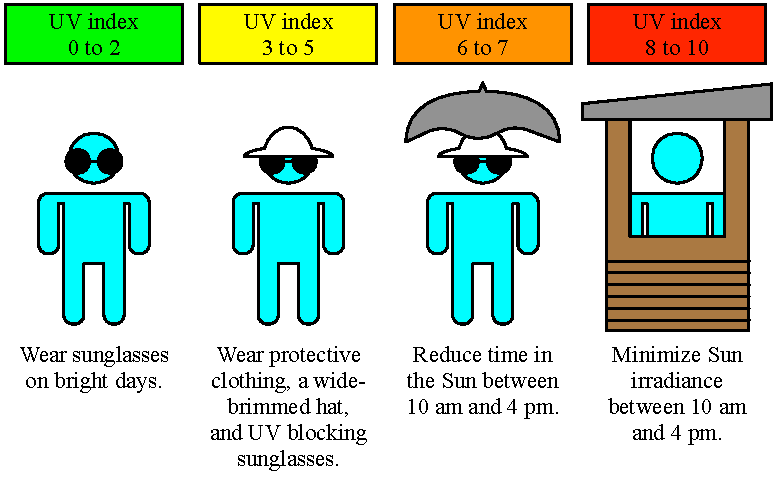
\includegraphics[width=1.0\hsize]{Figures/UVI_guideline.pdf}
\caption{Guidelines to protect oneself from overexposure to UV irradiance (US Environmental Protection Agency.)}
\label{fig:guidelines}
\vskip -10pt
\end{figure}
% Need more scientific information considering individual's characteristics
\textcolor{red}{Scientifically, the maximum UV exposure time is determined by the cumulative UV exposure as well as individual's characteristics such as skin type and the use of sunscreen lotions, which makes it even more complicated to get without using any UV measurement tools and technologies. In addition, the cumulative UV exposure is varying even on the position of the body and angle to the Sun. Thus it is crucial to directly measure the actual UV irradiance and cumulative irradiance on the skin area of interest by attaching the proper measurement tool on the skin area of interest. However, as fas as we concern, existing UV measurement tools are not useful for this purpose. The details about the scientific impacts of UV irradiance to human skin considering the individual's characteristics, and existing UV measurement tools will be given at the later section.}

% Introducing SmartPatch with main contributions
\textcolor{red}{In this paper, we introduces SmartPatch, a solar powered  and patchable smart UV level meter that guides people to safely play outdoor activities without concerning about their skin damages. The proposed SmartPatch is supported by two key technologies. The first key technology is a storage-less and converter-less energy harvesting~\cite{Lee:ASPDAC15} that does not require any battery nor voltage converter in energy harvesting logics. The second technology is a switch-less user interface to minimize the form-factor as well as the implementation cost. Instead of using any switches, SmartPatch detects the pre-defined patterns of user-intended artificial UV-level changes on the sensor and then controls SmartPatch according to the generated patterns. All the proposed technologies are implemented in a single chip for achieving a patchable device with extremely low-cost and small form factor.\\
% 
The key functions of Smartpatch are 1) display the real-time UVI, 2) display the remaining time to avoid skin damage, and 3) execution mode change or parameter programming by the user's skin type and the SPF of sunscreen lotions using a proposed switch-less interface or user's Smartphone. The functionalities and usefulness of SmartPatch are verified by measuring the UV level on several positions of the body during the various types of outdoor activities.}

%%%%%%%%%%%%%%%%%%%%%%%%%%%%%%%%
\section{Backgrounds}
%%%%%%%%%%%%%%%%%%%%%%%%%%%%%%%%
\subsection{Basics of UV and Skin damage}

Among overall range of UV radiation approaching the Earth, only UVA (320 to 400 nm) and UVB (280 to 320 nm) reach ground and affect human and environments. UVA causes skin aging and wrinkling while UVB causes well-known skin damages such as erythema (redness of the skin), sunburn and skin cancer~\cite{Matsumura:TAP04}.

%Self protection of the skin [reduced]
\textcolor{red}{The human skin has an ability to protect itself from the UV irradiance by skin darkening and thickening.
When the skin is exposed to the UV radiation, the skin immediately produces a dark-coloured pigment (called melanin) that delays the skin damage to two to four times. The degree of darkening effects is different by the skin types~\cite{Harrison:Method02}.}

%%%%%%%%%%%%%%%%%%%%%%%%%%%%%%%%
%\section{UV irradiance}
%%%%%%%%%%%%%%%%%%%%%%%%%%%%%%%%

%Standard of UV irradiance: MED and UV Index
Therefore, it is required to make a standard for the impact of UV irradiance to human skin.
Minimal erythema dose (MED), which is widely used to assess skin sensitivity to the UV irradiance, is defined as the lowest UV irradiance that produces minimally perceptible erythema~\cite{Diffey:CPPM91}.
The relative effectiveness for the MED by the wavelength of UV radiation is defined and introduced by the International Commission on Illumination~\cite{CIE}.
Erythema effectiveness by the UVB is 10 to 100 times larger than the effectiveness by the UVA.
The Sun spectrum multiplied by the erythemal effectiveness is the effective UV spectrum, and a result integrated over the whole spectrum is the effective UV irradiance and used as a measure of the UV irradiance.
%
\begin{equation}
\text{Effective~UV~irradiance} = \int A(\lambda)E(\lambda) d \lambda
 \end{equation}
%
where $A(\lambda)$ is the Sun spectrum, and $E(\lambda)$ is the erythemal effectiveness by the wavelength.
UV index is obtained by dividing the effective UV irradiance by 25 $mW/m^2$~\cite{CIE}.


%Sunscreen and SPF
People use sunscreens to protect their skin from the skin damage by absorbing or reflecting the UVB radiation.
Sun protection factor (SPF) is defined as a number on a scale of rating the degree of protection provided by sunscreens calculating as a following equation,
%
\begin{equation}
\text{SPF} = \frac{\int A(\lambda)E(\lambda) d \lambda}{\int A(\lambda)E(\lambda) / \text{MPF}(\lambda) d \lambda}
 \end{equation}
%
where MPF means monochromatic protection factor.

A bigger number of SPF means high reduction of UV absorption and reduces chances of skin damage.
For example, a sunscreen with SPF 15 blocks 93\% of UV radiation and extends the time to produce erythema about 15 times longer.
Therefore, a sunscreen with a specific SPF does not completely block UV irradiance but filters a part of UV irradiance.
Such a filtering extends the outdoor activity time without skin damages.
However, UV irradiance is still accumulated in the skin even with a sunscreen regardless of the SPF, and it may eventually incur skin damages.

\textcolor{red}{As described, the maximum UV exposure time is known as a function of the skin type, realtime UVI and the use of a sunscreen SPF of a sunscreen as a following function:}
%
\begin{equation} \label{eq: max_exp_time}
\begin{split}
\text{Maximum~UV~exposure~time}
&= \frac{\text{MED}(\text{skin~type})}{\int A(\lambda)E(\lambda)  / \text{MPF}(\lambda) d \lambda} \\
&\approx \frac{\text{MED}(\text{skin~type})\times \text{SPF}}{\text{UV~index} \times 0.025~mW/m^2},
\end{split}
\end{equation}

A remaining UV exposure time before experiencing skin damages is obtained by subtracting accumulated UV irradiance from the MED:
%
\begin{equation}
\begin{split}
&\text{Remaining~UV~exposure~time} \\
&= \frac{\text{MED}(\text{skin~type}) - \int \int A(\lambda, t)E(\lambda) / \text{MPF}(\lambda) d \lambda dt}{\text{UV~index} \times 0.025~mW/m^2 \times 1/\text{SPF}}.
\end{split}
\end{equation}

\textcolor{red}{In summary, without supporting from the dedicated UV measurement tools, it is almost impossible to accurately measure and estimate the remaining time.}


\subsection{UV Meters}
\textcolor{red}{There are numerous portable devices that measure the current UV irradiance as shown in Fig.~\ref{fig:UVI_meters}(a).
These devices can only measure the instant UV level while the measurement of cumulative UV exposure is actually necessary in real-life. More advanced devices shown in Fig.~\ref{fig:UVI_meters}(b) additionally inform the result of the UV irradiance accumulation. They are capable of displaying instantaneous UVI and calculating the maximum UV exposure time based on the skin type and SPF.
However, these devices typically include a battery and should communicate with smartphones~\cite{Netatmo, Ultra} to check measured information as well as to configure the devices. In addition, the shapes of the devices are often a wrist strap, a watch, a pendant, or a badge, and such devices only measure the UV irradiance of limited position of the body. Even on a same position of the body, they do not show the exact amount of accumulated UV irradiance because every skin surface has a different perpendicular angle to the Sun and is subject to continuous shading change.}
%
As shown in Fig.~\ref{fig:UV_exposure_skin}, each skin area has different UV irradiance due to the angle to the Sun.
In addition, partial shading in different areas of the skin continuously occurs by trees, buildings, other body parts, clothes, and so forth. For instance, people often experience skin damages on their shoulders while the other skin areas are manageable even if the whole body has been exposed to the Sun.

Recently, a patchable UV meter has been introduced by a cosmetic company as shown in Fig.~\ref{fig:UVI_meters}(c)~\cite{LOreal}. It is powered by the user's mobile phone via Near Field Communication (NFC) and activated by UVA and UVB rays. However, powering from NFC is not capable of measuring cumulative UV irradiance while the user is performing various outdoor activities.

\begin{figure}
\centering
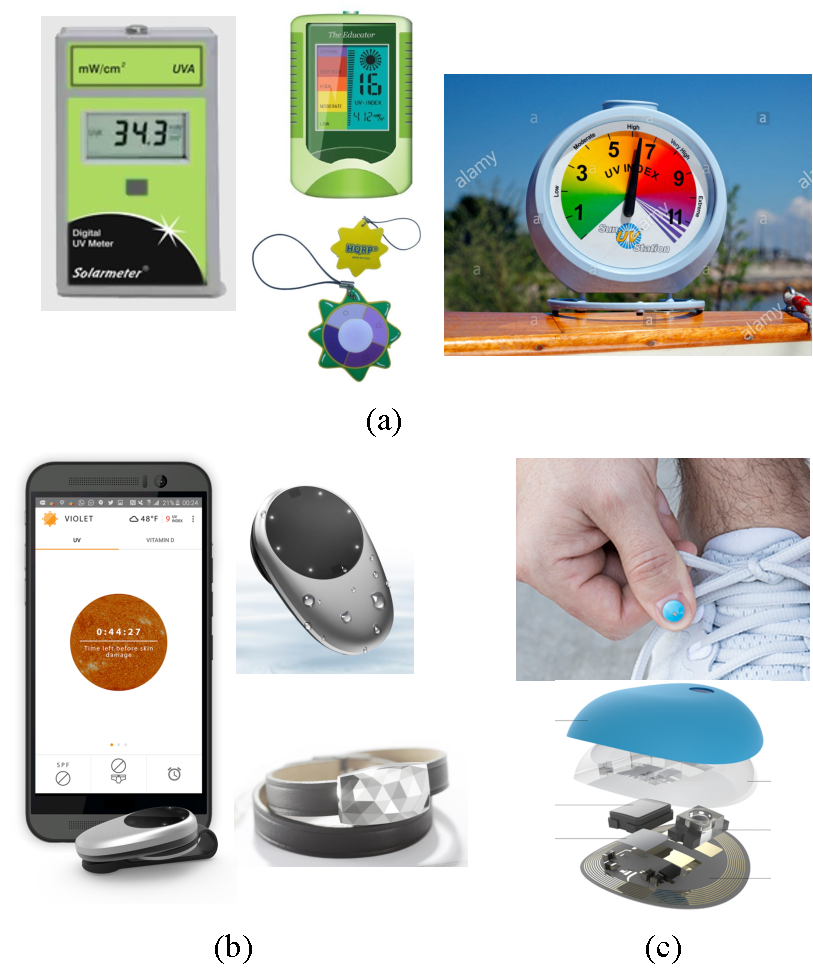
\includegraphics[width=0.8\hsize]{Figures/UVI_meter.pdf}
\caption{(a) Simple UV irradiance meters that inform the instantaneous UV irradiance level only and (b) advanced UV irradiance meters that calculate the maximum UV exposure time based on the skin type and the SPF of the sunscreen~\cite{Netatmo, Ultra, LOreal}.}
\label{fig:UVI_meters}
\end{figure}

\begin{figure}
\centering
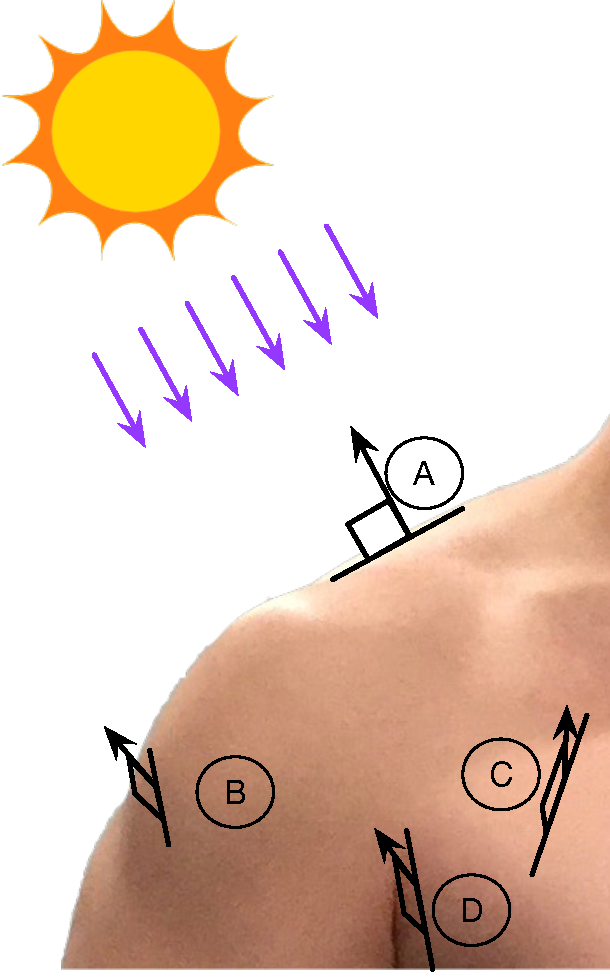
\includegraphics[width=0.4\hsize]{Figures/UV_skin_areas.pdf}
\caption{UV irradiance by the skin areas.}
\label{fig:UV_exposure_skin}
\end{figure}

%\textbf{A UV irradiance meter should be attached to a vulnerable skin area.}
Therefore, an accurate UV irradiance meter should position its UV sensor on the exact location of a particular skin with the same perpendicular angle to the Sun. However, it is not practical to mount a separate UV sensor from the measurement unit. A patchable design of a UV irradiance meter capable of measuring the cumulative UV irradiance can do this job. People generally figure out the most vulnerable skin area easily by the environment, their outfit and behavior. The UV irradiance meter can measure the actual cumulative UV irradiance by attaching to the vulnerable skin area \textcolor{red}{and our SmartPatch is designed to be efficiently attached to any interests of skin area that is the most vulnerable to the Sun.}

%%%%%%%%%%%%%%%%%%%%%%%%%%%%%%%%
\section{SmartPatch}
%%%%%%%%%%%%%%%%%%%%%%%%%%%%%%%%

Implementation of a patchable UV irradiance meter is challenging because of the form factor and weight.
Use of a battery is a common solution for the existing UV irradiance meters, but this method eventually ends of with a higher cost, a larger form factor and a heavy weight.

\textcolor{red}{SmartPatch is powered by storage-less and converter-less energy harvesting technique, which performs aggressive and rapid dynamic power management (DPM) and tracks the maximum power point (MPP)~\cite{Wang:ASPDAC14}. In addition, we develop a switch-less user interface for reducing the size and cost of SmartPatch. We take the following design considerations into account for SmartPatch.}

\begin{itemize}
\item Covering both the UVA and UVB spectrum,
\item Having a small form factor and possibly disposable,
\item \textcolor{red}{Programming the sunscreen SPF and user's skin type,}
\item Calculating the maximum UV exposure time based on the UV irradiance and skin type,
\item A patchable design to measure the actual cumulative UV irradiance on the exact skin area of interest,
\item Self-powered by a PV cell with the minimum possible size, and
\item No use of a power converter nor significant energy storage.
\end{itemize}

\subsection{Storage-less and converter-less Energy Harvesting Technology}
%\textbf{Storage-less and converter-less MPPT is the ultimate cross-layer power management for energy harvesting systems.}
Most energy harvesting systems adopt energy storage elements as well as power converters, which have been considered as must-have components for performing the maximum power point tracking (MPPT).
However, those components seriously limit the design in many aspects such as the weight, form factor, cost, maintainability, etc.
Recently, a breakthrough MPPT method that does not require power converters and energy storage elements has been introduced for high-efficiency PV energy harvesting applications~\cite{Wang:ASPDAC14}.

The basic principle of the storage-less and converter-less energy harvesting is to supply the harvested energy from the PV cell directly to the target device using a fine-grained DPM technique as shown in Fig.~\ref{fig:architectures}(b).
Power converter can be simply removed if the voltage level directly supplied from the PV cell is in the range of the operating voltage for the target device.
In general, the MPP voltage of the PV cell is maintained within a quite narrow range regardless of the solar irradiance.
This means that the PV cell generates almost-constant voltage output, that is a main role of power converters, as long as we keep the track of the MPP current.
Fast enough (or fine-grained) DPM makes the PV cell keep the MPP as if the current of the target device is a DC current as long as the average current is the same to the MPP current.
However, fast DPM may bring non-negligible energy and time overhead during the power state change, and finally the overall energy efficiency is degraded.
So a proper control method of the DPM considering the energy overhead is required for enlarging the energy efficiency.
We adopt a pulse width modulation (PWM) based DPM in designing of SmartPatch~\cite{Lee:ASPDAC15}.
The PWM based DPM controls the duty rate of power-on state compared with power-off state to keep the MPP.
This DPM achieves higher energy efficiency as well as the low implementation cost at the same time among various DPM architectures.

DPM is no longer available if the solar irradiance becomes too low, and SmartPatch should be completely shut down. The power management unit (PMU) detects power interruption and let the non-volatile RAM (NVRAM) save the necessary context \cite{Balsamo:TCAD16}. NVRAM is solely powered by the small size capacitor while it saves the context, and thus the proposed storage-less and converter-less MPPT allows to save only a very small capacity of context. Fortunately, SmartPatch needs to save just few bytes of information to the NVRAM.

\begin{figure}
\centering
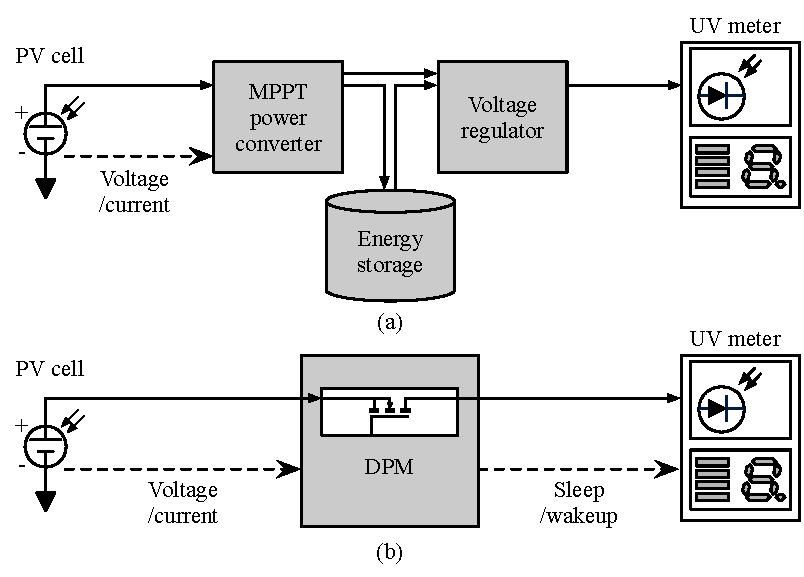
\includegraphics[width=1.0\hsize]{Figures/architectures.pdf}
\caption{(a) A typical architecture of an energy harvesting system and (b) a storage- and converter-less energy harvesting system~\cite{Wang:ASPDAC14}.}
\label{fig:architectures}
\end{figure}

A storage-less energy harvesting architecture raises relatively less technical challenges compared with the converter-less architecture. Instead, it may limit the area of the applications because the target devices become unavailable if the device is lack of harvested energy.
However, SmartPatch is one of the ideal applications of storage-less energy harvesting because it does not have to measure the UV irradiance when there is no sunlight.

\subsection{A switch-less user interface}
%\textbf{A switch-less user interface enables a low-cost disposable design and an extreme low-profile design.}
A switch (or button) is a necessary component for providing a function control to the users in most devices.
However, including a switch in a tiny device largely diminishes the advantages of a small, patchable and a very low-profile design.
These three requirements make the switch operation inconvenient and impose a serious design restriction.
We develop a switch-less user interface by detecting user generated unique patterns of the UV level change, which cannot be observed in the natural environmental change to the UV sensor and PV cell.

\begin{figure}
\centering
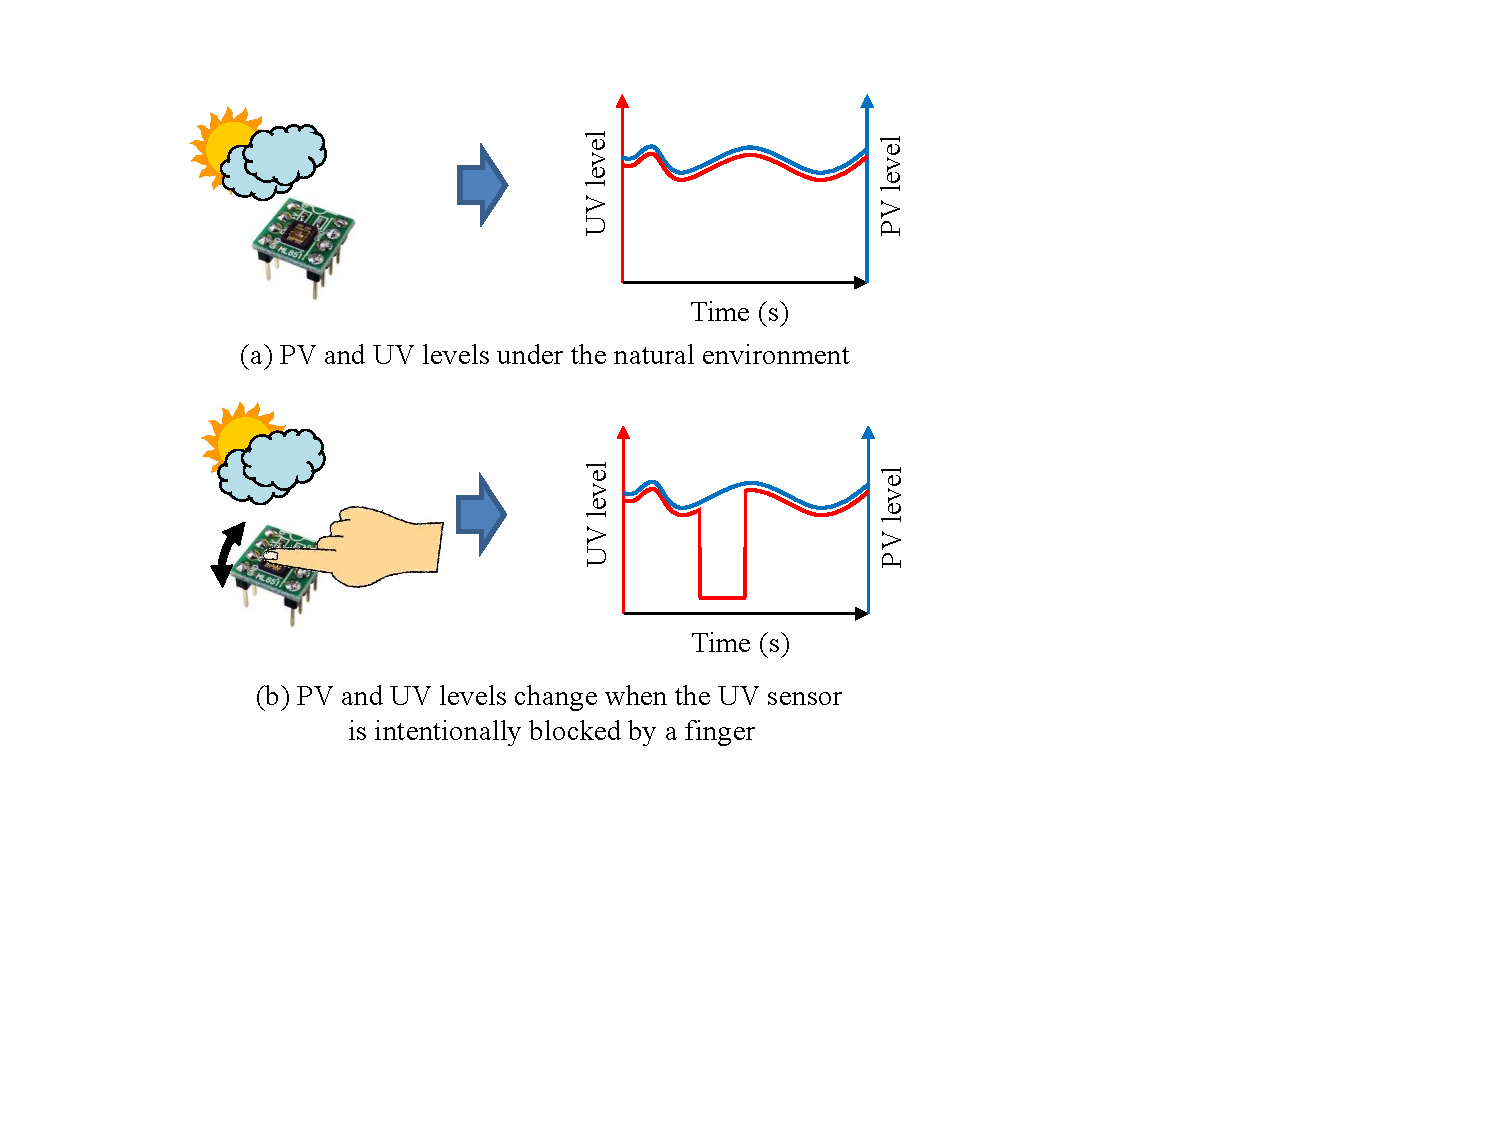
\includegraphics[width=0.8\hsize]{Figures/switchless_interface.pdf}
\caption{Principle of the switch-less interface.}
\label{fig:switchless_interface}
\end{figure}

Fig.~\ref{fig:switchless_interface} shows the principle of the operation of the proposed switch-less user interface.
A natural environmental change always makes both the UV level and PV level and they are highly correlated as shown in Fig.~\ref{fig:switchless_interface}(a).
The switch-less user interface action requires gently blocks on the UV sensor under a sufficient amount of Sunlight.
This makes the UV sensor output level is abruptly decreased as shown in Fig.~\ref{fig:switchless_interface}(b) while the PV cell generates enough power to operate SmartPatch.
This action is perceived as if there is a virtual switch and pressed by a finger.
A sequence and duration of the block and unblock actions of the UV sensor generate specific patterns.
A number of unique patterns perform various user interface functions such as skin type setting, resetting the device, etc.

\subsection{SmartPatch design}

We design a prototype of SmartPatch using two key technologies mentioned above.
Fig.~\ref{fig:block_diagram} shows a block diagram of the SmartPatch prototype consisting of a PV cell, a power management unit (PMU), control logic, a NVRAM, a UV sensor, a display, and other glue logic.
We implement the PMU with a PWM based DPM architecture.
The control logic includes a switch-less user interface.
The NVRAM stores the result of the UV irradiance accumulation, user skin type and use of a sunscreen.
The display is customized to show the current UV irradiance level as well as the remaining UV exposure time before experiencing skin damages.

\begin{figure}
\centering
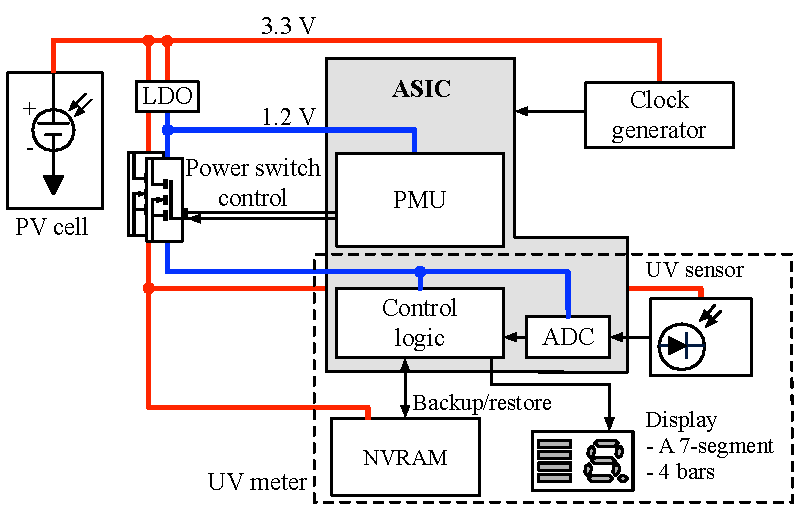
\includegraphics[width=1.0\hsize]{Figures/block_diagram.pdf}
\caption{A block diagram of SmartPatch.}
\label{fig:block_diagram}
\end{figure}

\begin{figure}
\centering
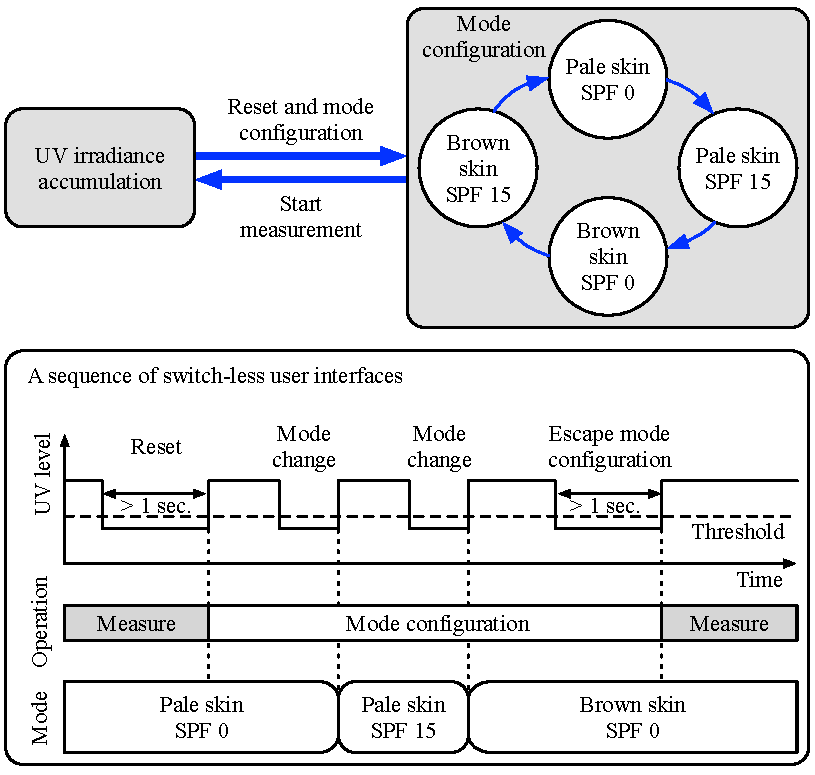
\includegraphics[width=1.0\hsize]{Figures/configuration.pdf}
\caption{Reset and mode configurations of SmartPatch.}
\label{fig:configuration}
\end{figure}

The current version of SmartPatch embeds two user interface functions: device reset and operation mode change.
Adding new features does not incur major design change.
Fig.~\ref{fig:configuration} shows examples of the switch-less user interface functions.
Blocking the UV sensor for more than a second resets SmartPatch and starts a new mode configuration.
\textcolor{red}{Then, the user is supposed to repeat the UV sensor blocking until the mode is set to a desired one. In the figure, the number of mode is four, but it can be easily changeable by using the NVRAM.
Repeating the reset motion -- blocking the UV sensor more than one second -- makes the device escape from the mode configuration and start a new UV irradiance accumulation.}

%%%%%%%%%%%%%%%%%%%%%%%%%%%%%%%%
\section{Single-chip implementation}
%%%%%%%%%%%%%%%%%%%%%%%%%%%%%%%%

%\textbf{A single-chip implementation is indispensable for the patchable design.}
The form factor is a crucial design consideration of the SmartPatch prototype.
We integrate most major parts of SmartPatch including the PMU into an application specific integrated circuit (ASIC.)
Table~\ref{table:fab_summary} shows the summary data of a single-chip fabrication.
The die size is 1.8 mm $\times$ 2.0 mm.
The number of equivalent logic gates used in the chip is only 817, which has a great potential to reduce the fabrication cost when it comes to a mass production.
The chip size is determined by the number of IOs in this case.
We look forward to having further reduction in the chip size by removing the redundant logic and IOs temporarily included for debugging purpose only.

\begin{table}
\centering
\caption{Summary of the single-chip fabrication.}
\label{table:fab_summary}
\begin{tabular}{|c|c|}  \hline
Parameters			&Values	\\ \hline \hline
Design technology		&SMIC 130 nm  \\ \hline
Supply voltage		&1.2 V (core) and 3.3 V (IO) \\ \hline
Chip size				&1.8 mm by 2.0 mm \\ \hline
\multirow{2}{*}{The number of IOs}		&15 (power), 8 (PMU), 19 (UV meter), \\
					&and 6 (debug purpose) \\ \hline		
The number of gates	&110 (PMU) and 707 (UV meter) \\ \hline
Maximum frequency	&160 kHz \\ \hline		
\end{tabular}
\end{table}

\begin{figure}
\centering
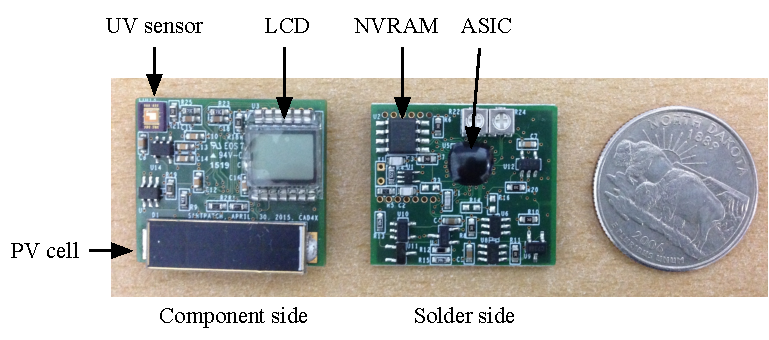
\includegraphics[width=1.0\hsize]{Figures/prototype.pdf}
\caption{A prototype of SmartPatch.}
\label{fig:prototype}
\end{figure}

Fig.~\ref{fig:prototype} shows the SmartPatch prototype implemented on a 23 mm $\times$ 22 mm board.
A custom LCD display, a PV cell and a UV sensor are on the component side of the board while the ASIC is on the solder side of the board as a chip on a board (COB) package with an NVRAM.
We add several discrete components on the both sides of the circuit board only for the debugging purpose for this version of prototype.
Table~\ref{table:prototype_summary} summarizes the implementation details of SmartPatch prototype.

\begin{table}
\centering
\caption{Summary of SmartPatch prototype.}
\label{table:prototype_summary}
\begin{tabular}{|c|c|}  \hline
Parameters			&Values	\\ \hline \hline
Size					&23 mm by 22 mm  \\ \hline
\multirow{2}{*}{Display information}	&Current UV index with one 7-segment and\\
					&remaining UV exposure time with four bars \\ \hline
User configuration		&2 skin types and use of a sunscreen (SPF 15) \\ \hline
\multirow{2}{*}{User interface}	&Reset and mode change  \\
					&by the switch-less user interface \\ \hline
Data preservation when 	&Backup and restore processes  \\
power is not enough	&with an NVRAM \\ \hline
\end{tabular}
\end{table}

Finally, we measure the power consumption of the prototype including the ASIC.
Table~\ref{table:power_summary} summarizes the power consumption of each component.
The ASIC itself consumes 1.6 mW while the other peripherals consume 6.4 mW.
In total, the prototype consumes 8 mW, which is low enough to use a small size PV cell (22 mm by 7 mm, 12.92 mW@$V_{MPP}$-3.4 V.)
A production-level implementation with a lower-power technology and a custom electronic ink display will make the power consumption several times lower.

The final implementation will have a single chip ASIC including the NVRAM, an e-ink display and the optimal-size of PV cell on a flexible PCB. This is being lead by a company through technology transfer.

\begin{table}
\centering
\caption{Power consumption of SmartPatch prototype.}
\label{table:power_summary}
\begin{tabular}{|c|c|c|}  \hline
Segment 			&Components					&Power (mW)	\\ \hline \hline
3.3 V for PMU		&Clock and IO pads			&1.9	\\ \hline
1.2 V for PMU 		&Digital and analog modules		&\multirow{2}{*}{1.6}		\\
and UV meter 	&in the ASIC chip 				&\\ \hline
3.3 V for peripherals & LCD, UV sensor and NVRAM	&4.5 \\ \hline

\end{tabular}
\end{table}

%\textbf{UV irradiance varies by the skin area.}
\begin{figure}
\centering
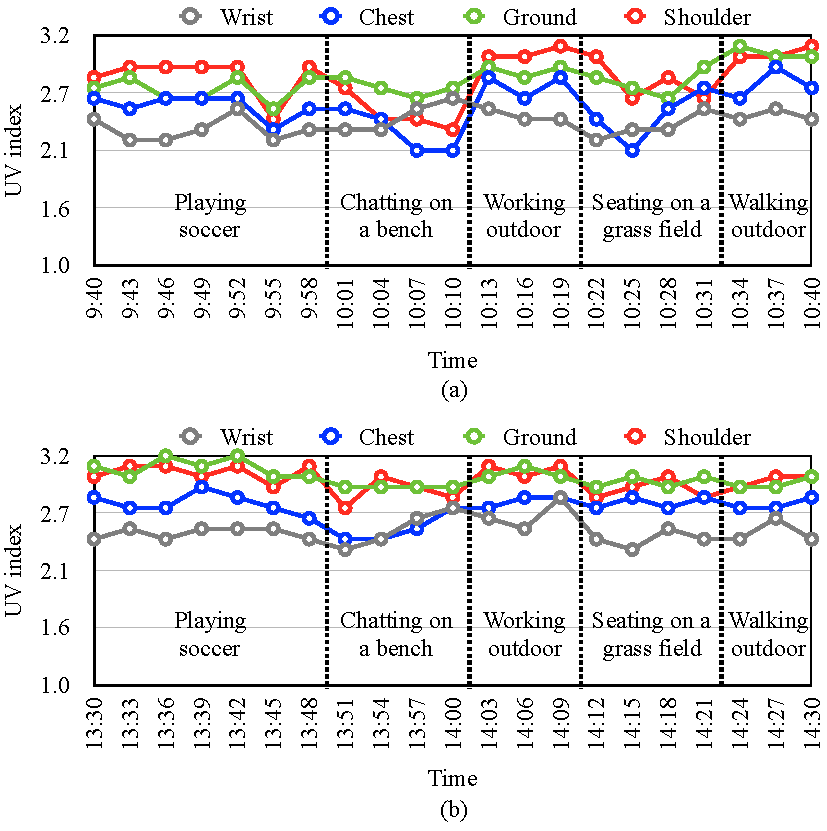
\includegraphics[width=1.0\hsize]{Figures/UV_measure.pdf}
\caption{Measurement results of UV irradiance by types of UV meters in the (a) morning and (b) afternoon.}
\label{fig:UV_measure}
\end{figure}

To verify the functionalities and usefulness of SmartPatch, we compare the UV irradiance on various skin areas in the morning and afternoon as shown in Fig.~\ref{fig:UV_measure}.
We measure UV irradiance on various skin areas in the morning and afternoon as shown in Fig. 9. \textcolor{red}{We measure the UV irradiance on the wrists, chests, shoulders, and the ground as a reference with SmartPatch (Fig.~\ref{fig:UV_measure}.)} The skin area of interest in the experiment is the shoulder, and SmartPatch is attached to the shoulder skin. Other UV meters are carried or attached as designed. For instance, a watch type UV meter measures the UV irradiance on the wrist. The UV irradiance to the ground increases by the angle to the Sun that is the maximum at 1:36 pm (13:36) in the experiments.

Of course, the UV irradiance to the skin area is different by activities.
For example, playing soccer, working and walking outdoor cause high UV irradiance to the shoulder and chest as shown in Fig.~\ref{fig:UV_measure}(a).
Unfortunately, the watch type UV meter on the wrist does not reflect the UV irradiance variation on the skin area of interest, i.e., shoulders, by the activities and the angle to the Sun.
However, it is impossible to put the watch type UV meter on the shoulder.
The UV irradiance to the shoulder is sometimes even larger than the UV irradiance to the ground when the shoulder has a perpendicular angle to the Sun.

%Impact of UV measurement error on the skin damage
We observe that existing UV meters under- or overestimate the accumulation of UV irradiance.
This implies that watch type UV meters underestimate UV accumulation on the shoulder up to 16\%, which may cause 50\% more chances of erythema symptoms if UV exposure lasts until the watch type UV meters indicate the maximum exposure time is over~\cite{Harrison:Method02}.

%%%%%%%%%%%%%%%%%%%%%%%%%%%%%%%%
\section{Conclusion}
%%%%%%%%%%%%%%%%%%%%%%%%%%%%%%%%

%\textbf{SmartPatch enables range of collaborative applications.}
The storage-less and converter-less MPPT can make a UV irradiance meter small enough to be patchable.
A patchable design can make the UV irradiance measurement directly on the skin area of interest, which greatly enhances the measurement accuracy.
SmartPatch can incorporate with sunscreen lotions, tanning oils, ski goggles, hats, and so on.
SmartPatch will open more proactive UV irradiance guideline for daily life.

%%%%%%%%%%%%%%%%%%%%%%%%%%%%%%%%
%% ACKNOWLEDGMENT%%%%%%%%%%%%%%%%%%
%%%%%%%%%%%%%%%%%%%%%%%%%%%%%%%%

%\section*{Acknowledgment}
%The authors would like to thank...

%%%%%%%%%%%%%%%%%%%%%%%%%%%%%%%%
%% REFERENCE%%%%%%%%%%%%%%%%%%%%%%%
%%%%%%%%%%%%%%%%%%%%%%%%%%%%%%%%

\bibliographystyle{ieeetr}
\bibliography{smartpatch}

%%%%%%%%%%%%%%%%%%%%%%%%%%%%%%%%
%% BIOGRAPHY%%%%%%%%%%%%%%%%%%%%%%%
%%%%%%%%%%%%%%%%%%%%%%%%%%%%%%%%

%\begin{IEEEbiography}[{\includegraphics[width=1in,height=1.25in,clip,keepaspectratio]{testing.pdf}}]{Donkyu Baek}
%Biography text here.
%\end{IEEEbiography}
%
%\begin{IEEEbiography}[{\includegraphics[width=1in,height=1.25in,clip,keepaspectratio]{testing.pdf}}]{Hyung Gyu Lee}
%Biography text here.
%\end{IEEEbiography}
%
%\begin{IEEEbiography}[{\includegraphics[width=1in,height=1.25in,clip,keepaspectratio]{testing.pdf}}]{Naehyuck Chang}
%Biography text here.
%\end{IEEEbiography}

%\vfill

\end{document}


